\section{Aufgabe1}
\label{sec:Aufgabe1}
%\lstinputlisting[language=Python, firstline=15, lastline=21]{plots/plot.py}
\subsection{Teilaufgabe a)}
Um die $10^5$ Signalereignisse mit der Transformationsmethode zu samplen wird
in Abbildung \ref{fig:Rechung} die Berechnung der Umkehrfunktion gezeigt.
\begin{figure}[h]
  \centering
  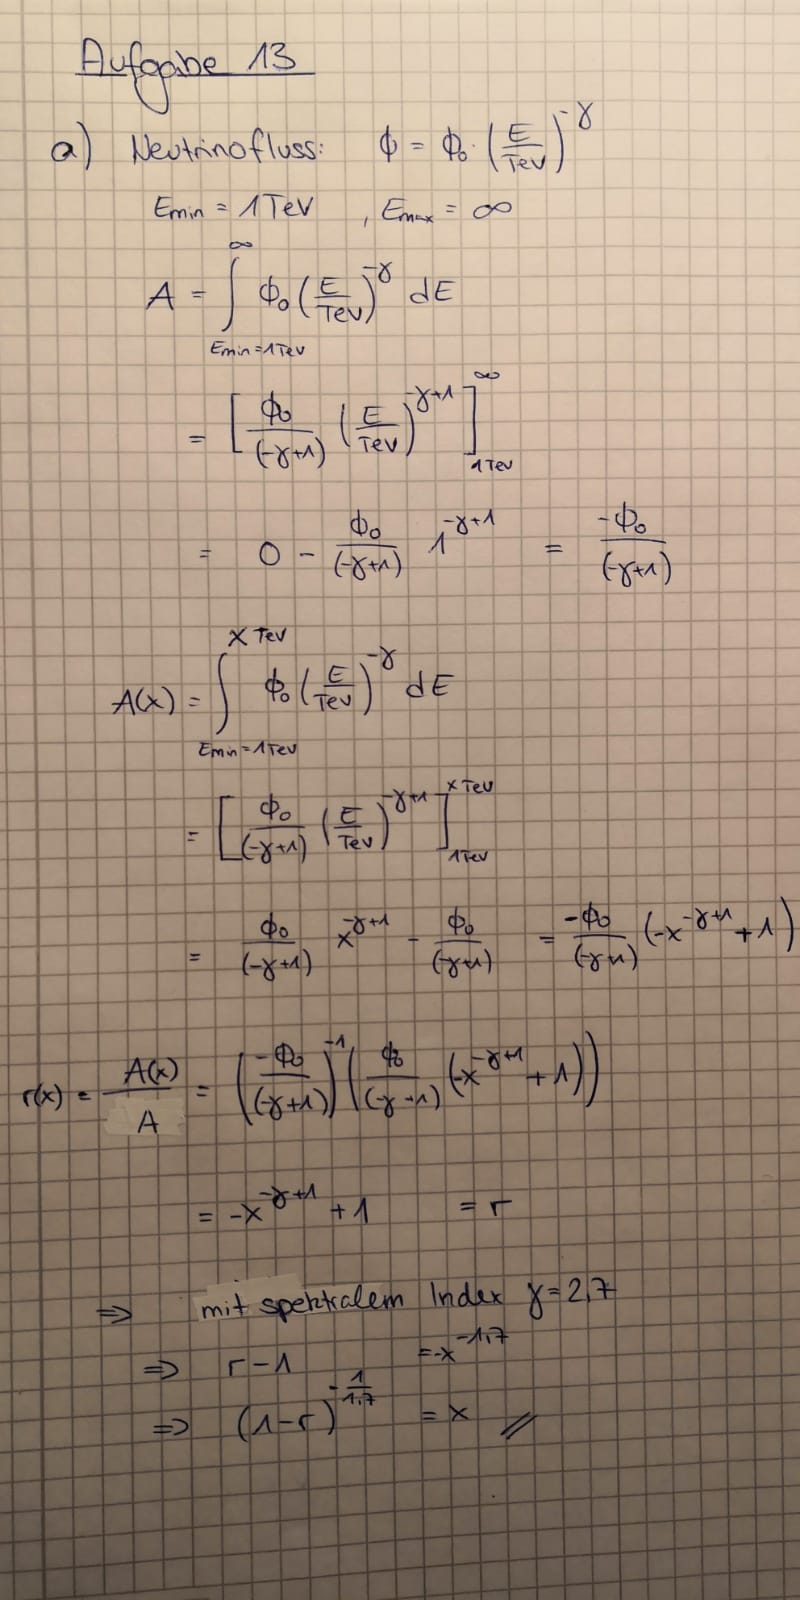
\includegraphics[height = 8cm]{pics/Blatt5_1a.jpeg}
  \caption{Berechnung der Transformationsmethode.}
  \label{fig:Rechnung}
\end{figure}
